\section{MindSqualls}\label{mindsqualls}
\mindsqualls er et .NET bibliotek til \legos NXT robotter.
\mindsqualls tillader kommunikation med NXT enheder via. Bluetooth og USB og fungerer ved at sende og modtager beskeder over disse to teknologier.
Biblioteket er skrevet i \csharp og kan dermed anvendes af alle de .NET kompatible sprog.

I det følgende afsnit gives en beskrivelse af bibliotekets struktur samt eksempler på anvendelse.

\paragraph{Abstraktion}
For at gøre det nemt at arbejde med NXT motorer og sensorer er der i \mindsqualls lavet en abstraktion over disse.
Hver type I/O er således implementeret i hver sin klasse med passende funktioner.
\Cref{mindsqualls:structure} viser et klassediagram, der beskriver relationerne mellem de primære klasser i \mindsqualls biblioteket.
Herunder gives en kort gennemgang af de primære klasser i \mindsqualls.

\begin{figure}
\centering
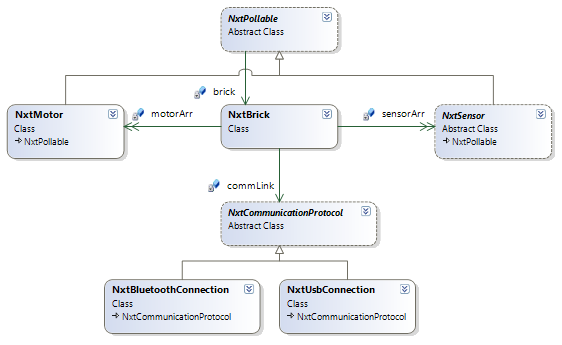
\includegraphics[width=0.8\textwidth]{mindsqualls}
\caption{Den overordnede \mindsqualls struktur}
\label{mindsqualls:structure}
\end{figure}

\subsection{NXT kommunikation}
\mindsqualls opretter forbindelse til NXT enheden vha. klassen \lstinline[style=csharp]!NxtCommunicationProtocol!.
Klassen fungerer, som navnet indikerer, som en protokol ved at definere en række abstrakte funktioner;
Der kan oprettes forbindelse til NXT enheden.
Denne kan afbrydes igen, og det kan til enhver tid fastslås om der er forbindelse til enheden.
Selve kommunikationen sker via kald til funktionen \lstinline[style=csharp]!Send! der tager et array af bytes som input og giver et array af bytes som output.
Altså kan funktionen både sende og modtage beskeder til og fra enheden.
Ved at lave specialiseringer af \lstinline[style=csharp]!NxtCommunicationProtocol! klassen, der definere disse funktioner, kan der kommunikeres med NXT enheden.
Der findes i \mindsqualls to specialiseringer af protokollen;
\begin{itemize}
\item \lstinline[style=csharp]!NxtUsbConnection!\\
Tillader kommunikation via USB (kablet)
\item \lstinline[style=csharp]!NxtBluetoothConnection!\\
Tillader kommunikation via Bluetooth (trådløst)
\end{itemize}

\subsection{NXT enheden}
I \mindsqualls er der lavet en abstraktion over selve NXT'en i form af klassen \lstinline[style=csharp]!NxtBrick!.
Som beskrevet herover kan der oprettes forbindelse mellem en computer og NXT enheden vha. USB eller Bluetooth.
Hvilken type forbindelse der skal benyttes angives i constructoren for \lstinline[style=csharp]!NxtBrick!.
Dette gøres med det første argument, som er en \lstinline[style=csharp]!enum! af typen \lstinline[style=csharp]!NxtCommLinkType!.
Der skal desuden angives et portnummer, som benyttes hvis der oprettes forbindelse via Bluetooth.

\begin{lstlisting}[style=csharpsmall,caption={Forbindelse til NXT enheder},label=mindsqualls:connect]
NxtBrick brickBT = new NxtBrick(NxtCommLinkType.Bluetooth, 16);
NxtBrick brickUSB = new NxtBrick(NxtCommLinkType.USB, 0);

brickBT.MotorA = ...
brickBT.Sensor1 = ...

brickBT.Connect();
// Kommunikation med enheden
brickBT.Disconnect();
\end{lstlisting}

I \cref{mindsqualls:connect} ses to eksempler på hvordan der skal oprettes forbindelse til enheden.
Selve forbindelsen oprettes ved kald til funktionen \lstinline[style=csharp]!Connect()! og afbrydes igen med \lstinline[style=csharp]!Disconnect()!.
Sensorer kan ''kobles'' til enheden ved de fire properties \lstinline[style=csharp]!Sensor1!, \lstinline[style=csharp]!Sensor2!, \lstinline[style=csharp]!Sensor3! og \lstinline[style=csharp]!Sensor4!.
Motorer anvender istedet \lstinline[style=csharp]!MotorA!, \lstinline[style=csharp]!MotorB! og \lstinline[style=csharp]!MotorC!.
Alle disse properties afspejler direkte den fysiske NXT enhed.
I \cref{mindsqualls:polling} er et eksempel på hvordan en sensor ''kobles'' til en enhed.

Når \lstinline[style=csharp]!Connect()! funktionen kaldes initialiseres enhedens tilknyttede sensorer.
Hvis man først knytter sensorer til enheden efter der er oprettet forbindelse, kaldes funktionen \lstinline[style=csharp]!InitSensors()! der sikrer at de nyligt tilknyttede sensorer er initialiserede.

\subsection{Input og Output}
For hver af de sensorer og motorer \lego producerer findes der i \mindsqualls en tilsvarende sensor.
Disse arver alle fra klassen \lstinline[style=csharp]!NxtPollable! der definerer metoder til at læse værdier fra de forskellige komponenter.
Dette gøres ved et \emph{Poll} der opdaterer den enkelte klasses tilstand således at den svarer til det fysiske komponent.
Samtidig er der for \lstinline[style=csharp]!NxtPollable! implementeret parallel automatisk polling.
Altså er det muligt automatisk at opdatere et komponents status.
Brugen af polling (både manuel og automatisk) kan ses i \cref{mindsqualls:polling}.
Her ses det også at polling er implementeret med et event der smides hver gang \lstinline[style=csharp]!Poll! kaldes.
I eksemplet er eventhandleren implementeret med et lambda udtryk der udskriver tilstanden for sensoren.

\begin{lstlisting}[style=csharpsmall,caption={Et eksempel på polling i \mindsqualls},label=mindsqualls:polling]
NxtUltrasonicSensor sonar = new NxtUltrasonicSensor();

sonar.OnPolled += pollable =>
    Console.WriteLine("Distance: {0}", sonar.DistanceCm);

brick.Sensor1 = sonar;

sonar.Poll();
// eller
sonar.PollInterval = 1000;
\end{lstlisting}

\subsubsection{Brug af sensorer}
Som et eksempel på brugen af sensor-klasser betragtes \legos ultralyds sensor (\cref{sensor:ultrasonic_sensor}), som er repræsenteret ved klassen \lstinline[style=csharp]!NxtUltrasonicSensor!.
Denne har en property \lstinline[style=csharp]!DistanceCm! der, som navnet angiver, returnerer afstanden fra sensoren til det objekt der er foran den.
I \cref{mindsqualls:polling} ses et eksempel på hvordan en sådan sensor oprettes og forbindes til NXT'en.

\subsubsection{Brug af motorer}
\legoms Servo Motoren er både en aktuator og en sensor, hvorfor det er muligt både at aflæse motorens nuværende position (med position menes der ændringen i grader ift. udgangspunktet), eller at sende kommandoer til at manipulere den nuværende position.

Til at aflæse løbende opdateringen, bruges samme metode som til aflæsning af de andre sensorer, via \textit{Polling}.

De vigtigste metoder til styring af motoren kan ses i brug i \cref{mindsqualls:motor}.
Her initialiseres en ny motor, hvorefter den roterer en hel omgang (360 grader), med hastighedsniveau 50 (som går fra 0 til 127).
Hvorefter den ny position bliver aflæst og skrevet til konsollen.

\begin{lstlisting}[style=csharpsmall,caption={Et eksempel på brug af en motor i \mindsqualls},label=mindsqualls:motor]
NxtMotor motor = new NxtMotor();
brick.MotorA = motor;

motor.Run(20, 360);
motor.Brake();

Console.WriteLine("Position: {0}", motor.TachoCount ?? 0);
\end{lstlisting}

\subsubsection{Synkronisering af motorer}
